\lstinputlisting[language=bash,basicstyle=\small]{python_codes/fieldstone_68/keywords}

\begin{center}
Code at \url{https://github.com/cedrict/fieldstone/tree/master/python_codes/fieldstone_68}
\end{center}

\par\noindent\rule{\textwidth}{0.4pt}

%%%%%%%%%%%%%%%%%%%%%%%%%%%%%%%%%%%%%%%%%%%%%%%%%%%%%%%%%%%%%%%%%%%%%%%%%%%%%%%%%%%%%%%%%%%%%%%%%%%%


\Literature: \cite{vack08}\cite{syva10}\cite{vakn12}


%------------------------------------------------------------
\subsubsection*{Description of the setup and benchmark cases}


The domain is $660\text{km}\times 600\text{km}$. 

\begin{center}
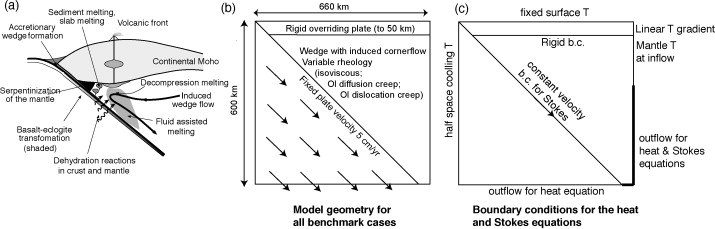
\includegraphics[width=14cm]{python_codes/fieldstone_68/images/fig1}\\
{\captionfont Taken from van Keken et al (2008) \cite{vack08}.
(a) Cartoon of the cornerflow model for subduction zone dynamics. 
(b) Benchmark geometry of a kinematic slab driving flow in the viscous
mantle wedge below a rigid overriding plate. 
(c) Boundary conditions for Stokes and temperature equations.}
\end{center}

As shown in the figure above, 
the inflow boundaries (at both wedge and trench sides) and top of the model 
have prescribed temperature. The wedge is assumed to be an incompressible fluid that
is driven only by the kinematic forcing of the slab. The wedge is
confined by the top of the slab and the base of the rigid overriding
plate (located at a depth of $50\text{km}$). 
The boundary conditions for the wedge are no-slip below the overriding plate and constant velocity
along the top of the slab. The velocity boundary conditions for the
boundaries of the wedge are either provided by the Batchelor cornerflow 
solution (cases 1a and 1b) or based on free inflow/outflow
boundaries (cases 1c, 2a, 2b). The velocity field is discontinuous between the slab
and the overriding plate.
The velocity in the slab is constant (5cm/yr) and it dips at a $45\degree$ angle
There is no radiogenic of shear heating.
The mantle wedge rheology is either linear viscous (cases 1a,b,c),
diffusion creep (case 2a) or dislocation creep (case 2b).





%___________________
\paragraph{Case 1a} The Stokes equations are not solved. Instead the velocity field
is prescribed analytically everywhere in the domain, using the corner flow solution 
in the mantle wedge. 

%___________________
\paragraph{Case 1b - dynamical flow in isoviscous wedge I}
This case is the same as 1a, except that the solution
for the wedge flow is determined by solving the Stokes equations while the Batchelor solution is
imposed on the inflow and outflow boundaries. This case tests the ability of the numerical method
to accurately reproduce the corner flow solution.



%___________________
\paragraph{Case 1c - dynamical flow in isoviscous wedge II} 
Same as case 1b, but with stress-free boundary conditions on the mantle wedge.



%___________________
\paragraph{Case 2a}

This case is the same as 1c, except that the viscosity of the wedge
is given by 
\[
\eta_{\text{diff,eff}} = \left( \frac{1}{\eta_{\text{diff}}} + \frac{1}{\eta_{\text{max}}} \right)^{-1}
\]
and
\[
\eta_{\text{diff}}=A_{\text{diff}} \exp\left( \frac{Q_{\text{diff}}}{RT} \right)
\]
with
$Q_{diff}=335kJ/mol$ and $A_{diff}=1.32043 \cdot 10^9Pa\cdot s$. $\eta_{max}=10^{26}$Pa.s

%___________________
\paragraph{Case 2b}

This case is the same as 1c, except that the viscosity of the wedge
is given by 
\[
\eta_{\text{disl,eff}} = \left( \frac{1}{\eta_{\text{disl}}} + \frac{1}{\eta_{\text{max}}} \right)^{-1}
\]
and
\[
\eta_{\text{disl}}=
A_{\text{disl}} \dot\varepsilon^{(1-n)/n} \exp \left( \frac{Q_{\text{disl}}}{nRT} \right)
\]
with $Q_{\text{disl}}=540kJ/mol$, $n=3.5$ and $A_{\text{disl}}=28968.6Pa\cdot s^{1/n}$. 
$\eta_{\text{max}}=10^{26}$Pa.s


%------------------------------------------------------------
\subsubsection*{Description of the code}

The mesh is built using Gmsh \cite{gere09}. IRIS:describe here how. 

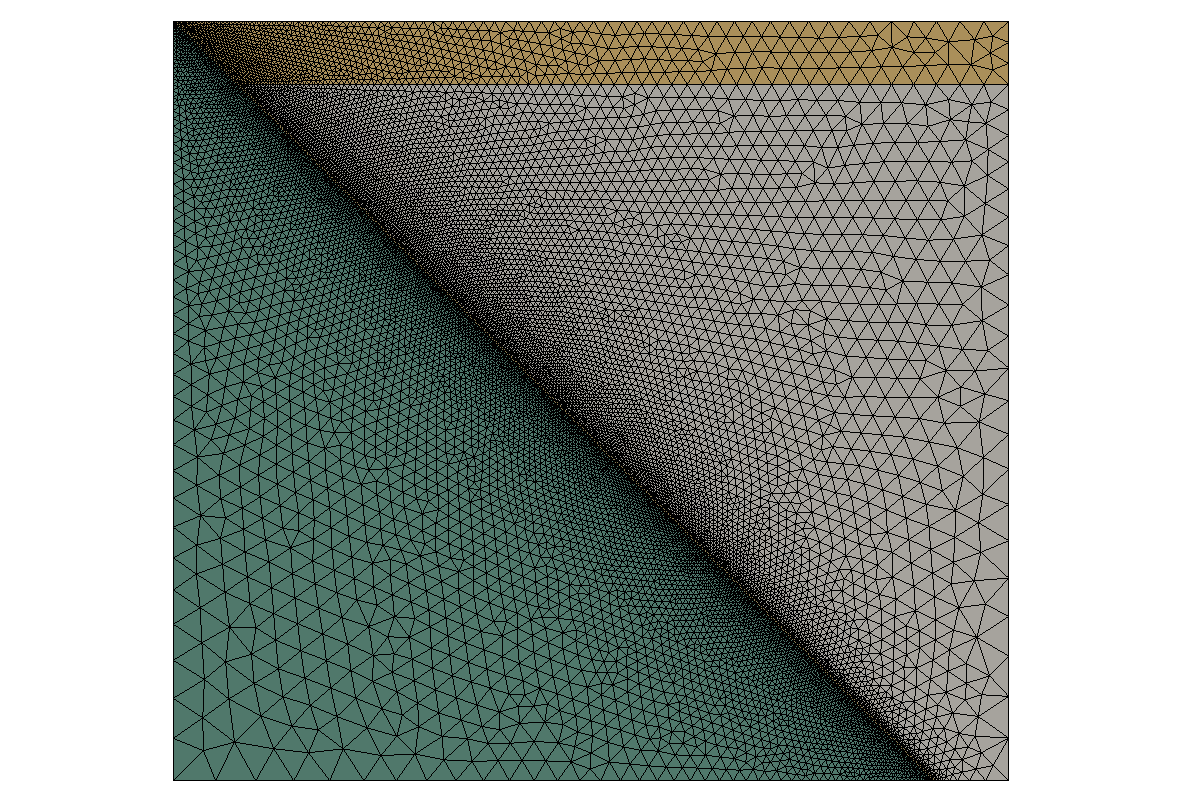
\includegraphics[width=7cm]{python_codes/fieldstone_68/images/mesh1}
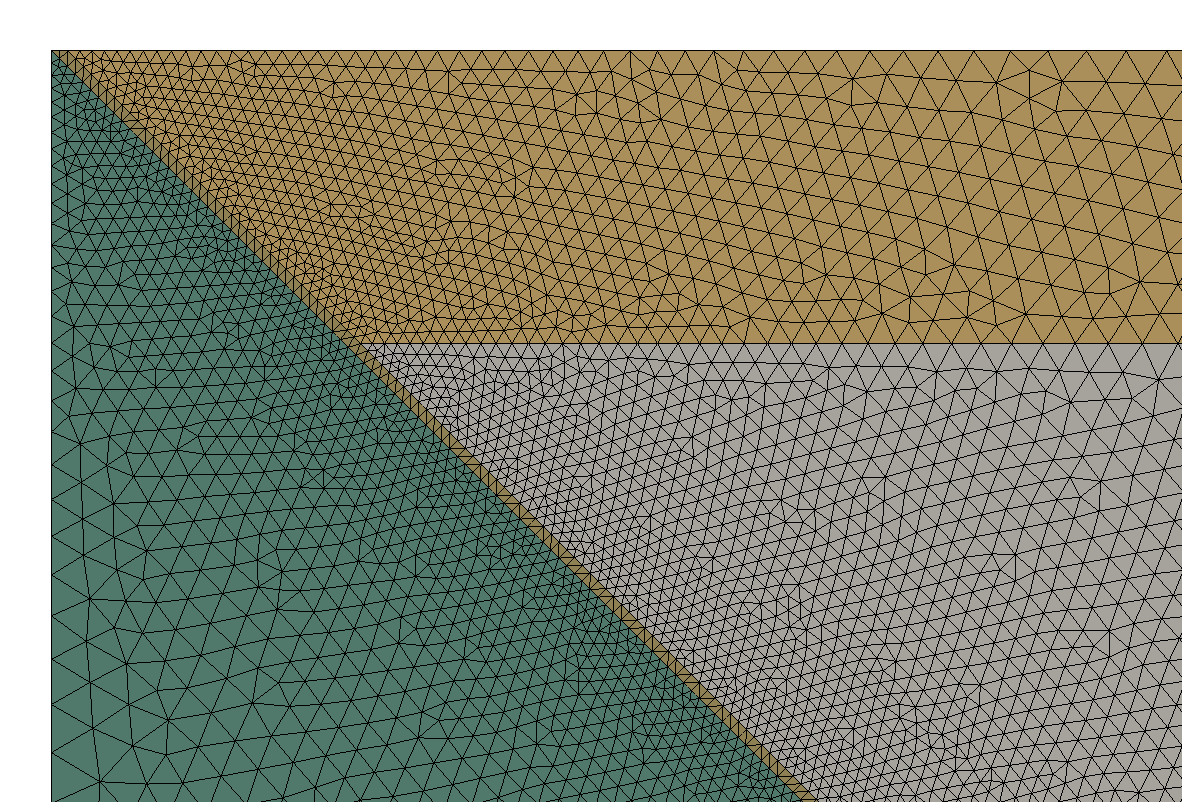
\includegraphics[width=7cm]{python_codes/fieldstone_68/images/mesh2}

Crouzeix-Raviart elements are used for the Stokes equations and $P_2$ elements are 
used for the temperature. 

\begin{center}
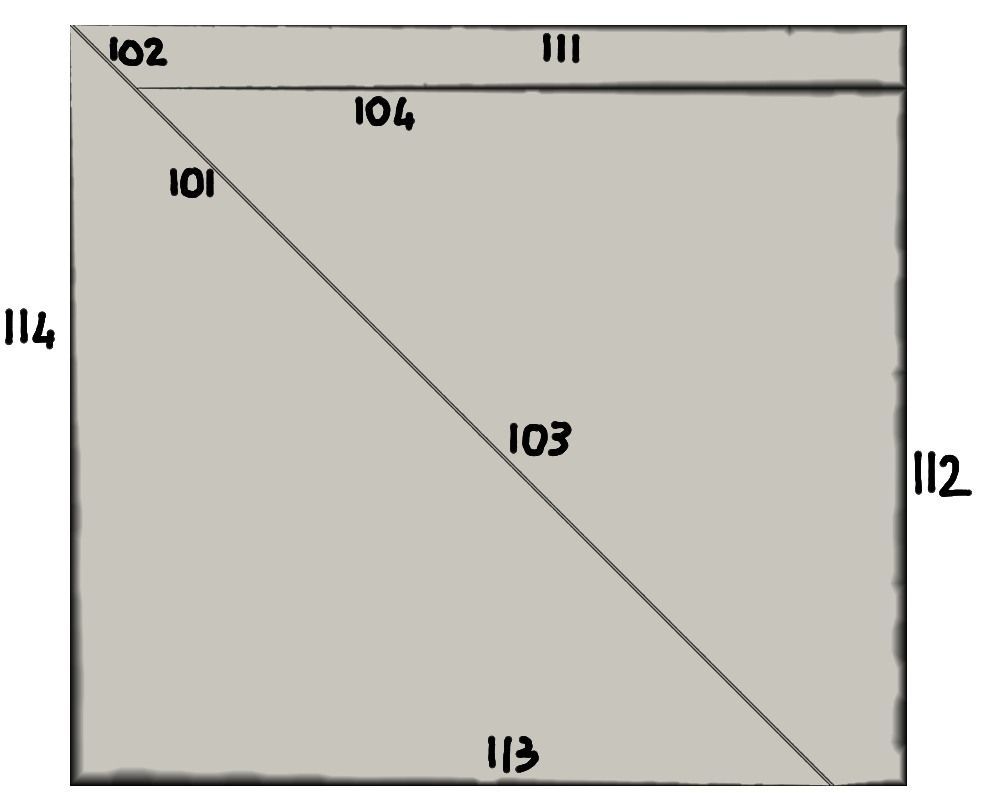
\includegraphics[width=7cm]{python_codes/fieldstone_68/images/interfaces}
\end{center}


In order to determine whether a point is inside a triangle, we assume that 
the reduced coordinates $r,s$ exist and satisfy the following 
relationships:
\begin{eqnarray}
x &=& N_1(r,s) x_1 + N_2(r,s) x_2 + N_3(r,s) x_3 \nn\\  
y &=& N_1(r,s) y_1 + N_2(r,s) y_2 + N_3(r,s) y_3 \nn
\end{eqnarray}
where $N_i$ are the linear basis functions inside a triangle, see Section~\ref{ss:p1}.

We also have the property that $N_1+N_2+N_3=1$ everywhere inside the element, so that 
we now have a system of 3 equations for our three unknowns $N_1$, $N_2$ and $N_3$ (having
obtained these, we can later easily find $r$ and $s$).
We must then solve:
\begin{eqnarray}
x &=& N_1 x_1 + N_2 x_2 + N_3 x_3 \nn\\  
y &=& N_1 y_1 + N_2 y_2 + N_3 y_3 \nn\\
0 &=& N_1+N_2+N_3 \nn
\end{eqnarray}
which yields
\[
N_1=\frac{(y_2 - y_3)(x - x_3) + (x_3 - x_2)(y - y_3)}{(y_2 - y_3)(x_1 - x_3) + (x_3 - x_2)(y_1 - y_3)}
\qquad
N_2=\frac{(y_3 - y_1)(x - x_3) + (x_1 - x_3)(y - y_3)}{(y_2 - y_3)(x_1 - x_3) + (x_3 - x_2)(y_1 - y_3)}
\qquad
N_3=1-a-b
\]
and then $r=N_2$ and $s=N_3$



%------------------------------------------------------------
\subsubsection*{Results}


%_______________________
\paragraph{Cases 1a,b,c}. 

\begin{center}
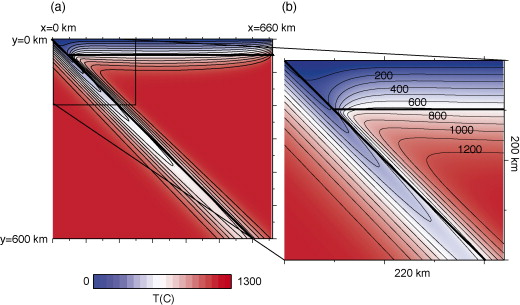
\includegraphics[width=14cm]{python_codes/fieldstone_68/images/fig2}\\
{\captionfont Taken from \cite{vack08}. Temperature prediction for case 1a. 
The bold lines indicate the top of the slab and base of the overriding plate. 
(b) Close up of the top left part of the model.}
\end{center}

\begin{center}
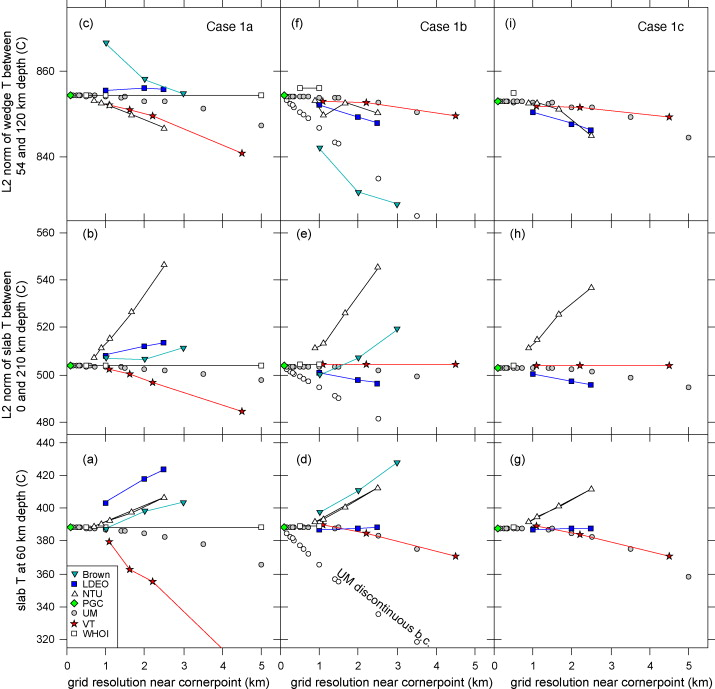
\includegraphics[width=14cm]{python_codes/fieldstone_68/images/fig3}\\
{\captionfont Taken from \cite{vack08}. 
Predictions for selected thermal properties for the isoviscous benchmark cases 1a 
(frames a-c), 1b (d-f) and 1c (g-i). The quantities represent a spot measurement at
the slab–wedge interface at 60 km depth (frames a, d, g), the average temperature 
along the slab–wedge interface from 0 to 210 km depth (frames b, e, h), and the
average temperature in a triangular portion of the wedge (frames c, f, i). 
The averages are computed with an L2 norm from an equidistant grid with 6 km spacing.
}
\end{center}
 
%_______________________
\paragraph{Cases 2a,b}.

\begin{center}
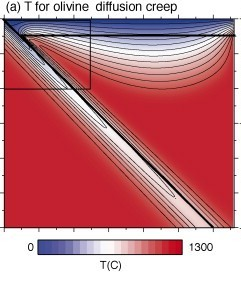
\includegraphics[width=14cm]{python_codes/fieldstone_68/images/fig4}\\
{\captionfont Taken from \cite{vack08}. 
(a) Temperature prediction for case 2a with olivine diffusion creep in 
the mantle wedge. (b) Close up of the top left part of the model, as in Fig. 2b.
(c) Close up of the model with olivine dislocation creep in the mantle wedge.
}
\end{center}
 
